\chapter{\communicationname}

A continuación, se presenta una revisión literaria de las comunicaciones cuánticas, facilitando comprender la relevancia e implicaciones de este campo de estudio.

\section{Metodología}

Esta sección documenta cada etapa del proceso seguido con la finalidad de mostrar de forma transparente cómo se llevó a cabo esta revisión sistemática de la literatura.

\begin{table}[H]
\centering
\caption[Protocolo PICOC - Ciberseguridad post cuántica]{%
    \vspace{4pt}
    \fontsize{12}{11}\selectfont \\
    Protocolo PICOC - Comunicaciones Cuánticas \\[2pt] % Tu subtítulo
}
\label{tab:protocolo_picoc_comunicaciones}
\begin{tabular}{@{} l p{10cm} @{}} % Changed L to p
\hline\hline
\textbf{Elemento} & \textbf{Descripción} \\
\hline
Población & Sistemas y redes de comunicación cuántica. \par\vspace{0.5pt} \\
\hline
Intervención & Tecnologías, arquitecturas y protocolos de transmisión de información cuántica. \par\vspace{0.5pt}\\
\hline
Comparación & Tecnologías de comunicación tradicionales y diferentes enfoques de desarrollo de comunicaciones cuánticas.\par\vspace{0.5pt} \\
\hline
Resultados & Métricas de calidad y rendimiento, la escalabilidad, los desafíos tecnológicos y operativos, y la viabilidad práctica de la implementación de la comunicación cuántica. \par\vspace{0.5pt}\\
\hline
Contexto & Evolución de infraestructuras y tecnologías para la transmisión de información en la era de comunicaciones cuánticas. \par\vspace{0.5pt}\\
\hline\hline
\end{tabular}
\end{table}

A continuación se presentan las preguntas de investigación definidas en esta revisión, las cuáles son el eje central de la investigación. Cada componente del protocolo está diseñado para contribuir directamente a la respuesta de estas preguntas, garantizando la coherencia y validez de los resultados.

\begin{itemize}
    \item \textbf{Q1:} ¿Qué tecnologías, arquitecturas y protocolos constituyen el estado del arte actual de las comunicaciones cuánticas?
    \item \textbf{Q2:} ¿Cuáles son los principales desafíos tecnológicos y físicos que dificultan el despliegue a gran escala de redes de comunicación cuántica?
    \item \textbf{Q3:} ¿Qué impacto potencial tienen las comunicaciones cuánticas en el desarrollo de las infraestructuras de comunicación, y en qué medida podrían transformar los fundamentos tecnológicos que rigen las comunicaciones actuales?
    \item \textbf{Q4:} ¿Cuáles son los casos de uso industriales relevantes para las comunicaciones clásicas y cuánticas?
\end{itemize}

Con el objetivo de construir una cadena de búsqueda que permitiera identificar la máxima literatura relevante, se definió la siguiente terminología clave y sus sinónimos correspondientes.

\begin{table}[H]
\centering
\caption[Palabras clave - Comunicaciones Cuánticas]{
    \vspace{4pt}
    \fontsize{12}{11}\selectfont \\
    Palabras clave - Comunicaciones Cuánticas \\[2pt] % Nuevo título para esta tabla
}
\label{tab:keywords_comunicaciones_cuanticas} % Nueva etiqueta para esta tabla
\begin{tabular}{@{} l p{6cm} @{}} % Usamos 'l' para Keyword y 'p{6cm}' para Sinónimos con ancho fijo
\hline\hline
\textbf{Keyword} & \textbf{Sinónimos} \\
\hline
quantum communication & quantum communication systems \\
\hline
quantum networks & quantum network architecture \\
\hline
quantum internet & quantum channel \\
\hline
quantum key distribution & quantum key distribution, quantum key distribution systems, quantum key distribution protocols, QKD \\
\hline\hline
\end{tabular}
\end{table}

Posteriomente se diseñó una cadena de búsqueda basada en la terminología clave previamente definida, junto con una serie de filtros para delimitar los resultados. .

\begin{figure}[H]
\centering
\begin{minipage}{0.8\textwidth} % Puedes ajustar el ancho si es necesario
    \centering
    {\fontsize{12}{11}\selectfont % Mantiene el formato del título/subtítulo
    \textbf{Bloque de Código 4} \\ % Cambiado a BLOQUE DE CÓDIGO III
     Cadena de Búsqueda - Comunicaciones Cuánticas \\ % Cambiado para la nueva SLR
 }
  \begin{minted}[
  linenos=false, % Sin números de línea
      linenos=false,
        frame=single,
        framesep=2mm,
        bgcolor=lightgray!20,
        fontfamily=tt,
        fontsize=\small,
        obeytabs=true,
        tabsize=4
   ]{python}
TITLE-ABS-KEY (
  "Quantum Key Distribution" OR
  "Quantum Key Distribution Protocols" OR
  "Quantum Key Distribution Systems" OR "QKD"
)
AND TITLE-ABS-KEY (
  "Quantum Communication" OR
  "Quantum communication systems" OR
  "Quantum Networks" OR
  "Quantum network architecture" OR
  "Quantum Internet" OR
  "Quantum channel"
)
AND PUBYEAR > 2020 AND PUBYEAR < 2025
AND (LIMIT-TO(SRCTYPE, "j") OR LIMIT-TO(SRCTYPE, "p"))
AND (LIMIT-TO(SUBJAREA, "COMP") OR LIMIT-TO(SUBJAREA, "ENGI"))
AND (LIMIT-TO(DOCTYPE, "ar") OR LIMIT-TO(DOCTYPE, "cp"))
AND (LIMIT-TO(LANGUAGE, "English"))
   \end{minted}
\end{minipage}
\end{figure}

Adicional a la cadena de búsqueda empleada, se aplicaron filtros para
delimitar los resultados. Se restringió la búsqueda a: 
\begin{itemize}
    \item \textbf{Año de publicación}: 2020-2025
    \item \textbf{Idioma}: Inglés
    \item \textbf{Tipo de publicación}: artículos de revista, actas de congreso y \emph{pre-prints}
    \item \textbf{Área temática}: Ingeniería y Telecomunicaciones
\end{itemize}

Los artículos identificados a través de la estrategia de búsqueda fueron sometidos a un proceso de cribado basado en un conjunto de criterios de inclusión y exclusión. Esto permitió refinar la selección y asegurar que tan solo los estudios más pertinentes formaran parte de la selección final de artículos.

\begin{longtable}{@{} p{5.45cm} p{7.973cm} @{}}
\caption[Criterios - Comunicaciones Cuánticas]{
    \vspace{4pt}
    \fontsize{12}{11}\selectfont \\
    Criterios - Comunicaciones Cuánticas \\[2pt]
}
\label{tab:criterios_comunicaciones_cuanticas}\\
\hline
\noalign{\vskip 2pt}
\hline
\textbf{Inclusión} & \textbf{Exclusión} \\
\hline
\endfirsthead

\hline
\endhead

\hline
\endfoot

\hline
\noalign{\vskip 2pt}
\hline
\endlastfoot

% Primera "fila" de contenido para permitir el corte
\textbf{IC1:} El estudio se centra específicamente en sistemas de comunicación cuántica o redes cuánticas, incluyendo su diseño, arquitectura, componentes clave o implementación.\par\vspace{8pt}
\textbf{IC2:} El documento describe, propone, analiza o evalúa protocolos de comunicación cuántica o mecanismos de distribución de claves cuánticas.\par\vspace{8pt}
\textbf{IC3:} El artículo aborda desafíos tecnológicos y operativos relacionados con el despliegue de infraestructuras de comunicación cuántica.
&
\textbf{EC1:} Se excluyen estudios centrados exclusivamente en la computación cuántica o física cuántica fundamental sin implicación directa con la comunicación cuántica.\par\vspace{8pt}
\textbf{EC2:} Se excluyen estudios sobre comunicaciones o redes clásicas que no integren o discutan explícitamente tecnologías o el impacto directo de la comunicación y redes cuánticas.\par\vspace{8pt}
\textbf{EC3:} Se excluyen trabajos que se consideren que tienen una baja relevancia académica o no aportan una contribución significativa al campo de las comunicaciones cuánticas.\par\vspace{8pt}
\textbf{EC4:} Se excluirán los estudios que se centren exclusivamente en optimizaciones de componentes muy específicos de QKD sin abordar la implementación a nivel de sistema, protocolo o red de comunicaciones cuánticas.
\\
\hline

\textbf{IC4:} El estudio discute el impacto o transformación de las infraestructuras y fundamentos tecnológicos de las comunicaciones actuales debido a las tecnologías cuánticas.\par\vspace{8pt}
\textbf{IC5:} El artículo analiza casos de uso, aplicaciones industriales o escenarios de implementación práctica para las comunicaciones y redes cuánticas.
&
\textbf{EC5:} Se excluyen aquellos estudios que se limiten a la identificación o análisis de vulnerabilidades y ataques en comunicaciones cuánticas, sin aportar propuestas de solución o medidas de mitigación a nivel de sistema o red.\par\vspace{8pt}
\textbf{EC6:} Se excluirán los estudios limitados a demostraciones de laboratorio o simulaciones que no introduzcan mejoras sustanciales, análisis comparativos de arquitecturas ni consideraciones sobre integración o escalabilidad en redes cuánticas.
\\
\end{longtable}

\section{Modelo PRISMA}

Para estructurar y documentar de forma rigurosa el proceso de selección de estudios, se ha seguido la metodología PRISMA (Preferred Reporting Items for Systematic Reviews and Meta-Analyses). Este modelo proporciona una guía estandarizada que permite garantizar la transparencia, la reproducibilidad y la trazabilidad en revisiones sistemáticas, desde la fase de identificación de fuentes hasta la inclusión final de los estudios relevantes.

\begin{figure}[H]
\centering
\caption[Modelo PRISMA - Comunicaciones Cuánticas]{
    \vspace{4pt}
    \fontsize{12}{11}\selectfont \\
    Modelo PRISMA - Comunicaciones Cuánticas \\
}
\footnotesize Fuente: Elaboración propia
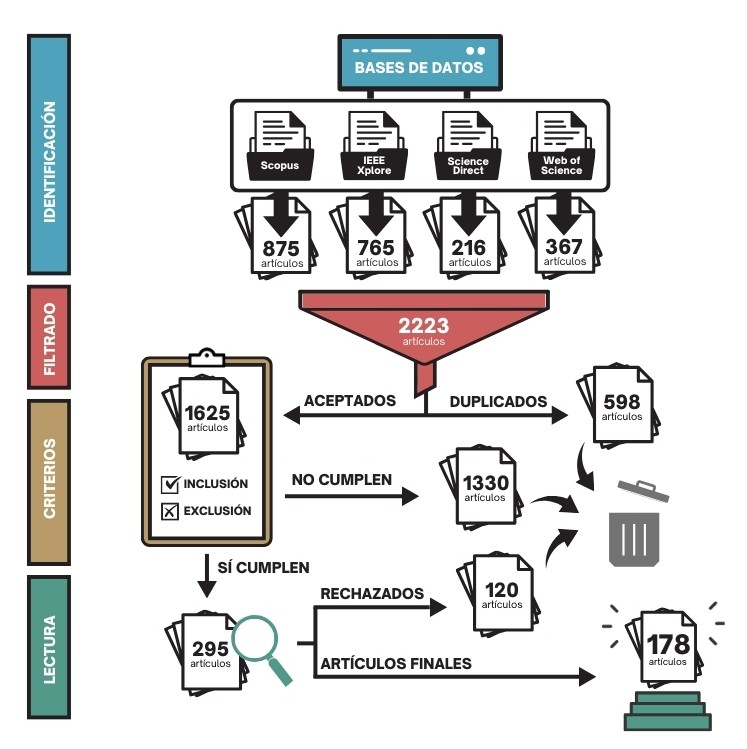
\includegraphics[width=0.85\textwidth]{pictures/Modelo_PRISMA_SLRCommunication.jpg}
\label{fig:modelo_prisma_SLRcomunica}
\end{figure}

Fueron recopilados 2223 artículos de las bases de datos académicas seleccionadas. Durante el proceso de filtración inicial se identificaron y eliminaron 598 artículos duplicados, dando como resultado 1625 artículos únicos. Posteriormente, estos artículos se analizaron conforme a unos criterios de inclusión/exclusión establecidos, tan solo 295 fueron aceptados. En la fase final se realizó una lectura completa y evaluación de calidad, conformando un conjunto de 178 artículos que constituyen los artículos finales de esta revisión sistemática.

\section{Análisis de Resultados}

Con la finalidad de comprender los resultados obtenidos en esta revisión, se realizó un análisis cuantitativo orientado a identificar tendencias, patrones y características relevantes.

La primera grafica corresponde al año de publicación y tipo de artículo, este análisis resulta especialmente relevante porque permite ver la evolución temporal de la producción científica en el campo de las comunicaciones cuántica.

\begin{figure}[H]
\centering
\caption[Año de publicación y tipo de artículo - Comunicaciones Cuánticas]{
    \vspace{4pt}
    \fontsize{12}{11}\selectfont \\
    Año y Tipo de publicación - Comunicaciones Cuánticas\\
}
\footnotesize Fuente: Elaboración propia
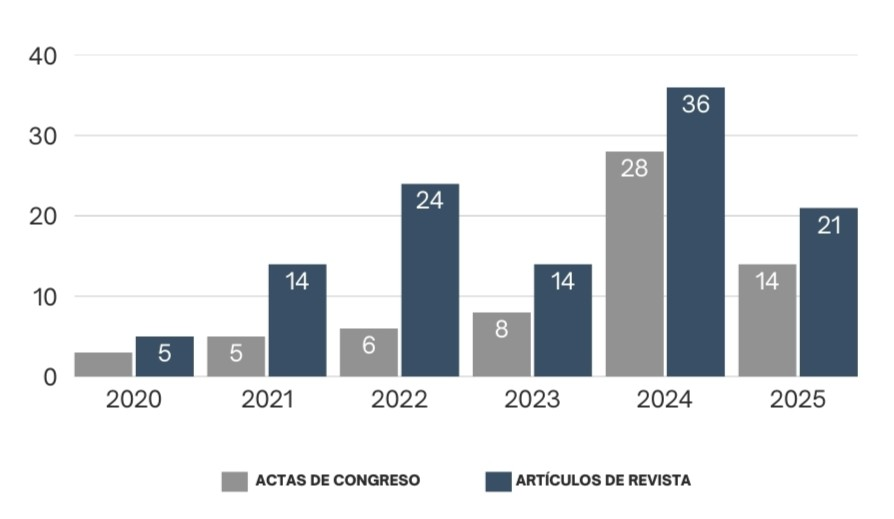
\includegraphics[width=0.95\textwidth]{pictures/Años_Tipos_SLRCommunication.jpg}
\label{fig:año_tipo_SLRcomunica}
\end{figure}

De manera complementaria, se realizó un análisis de las palabras clave más frecuentes. E enfoque permite observar qué términos y conceptos emergen con mayor recurrencia en la literatura y se obtiene una visión del vocabulario dominante que guía la actualidad de este campo académico.


\begin{figure}[H]
\centering
\caption[Frecuencia de palabras clave - Comunicaciones Cuánticas]{
    \vspace{4pt}
    \fontsize{12}{11}\selectfont \\
    Frecuencia de palabras clave - Comunicaciones Cuánticas \\
}
\footnotesize Fuente: Elaboración propia
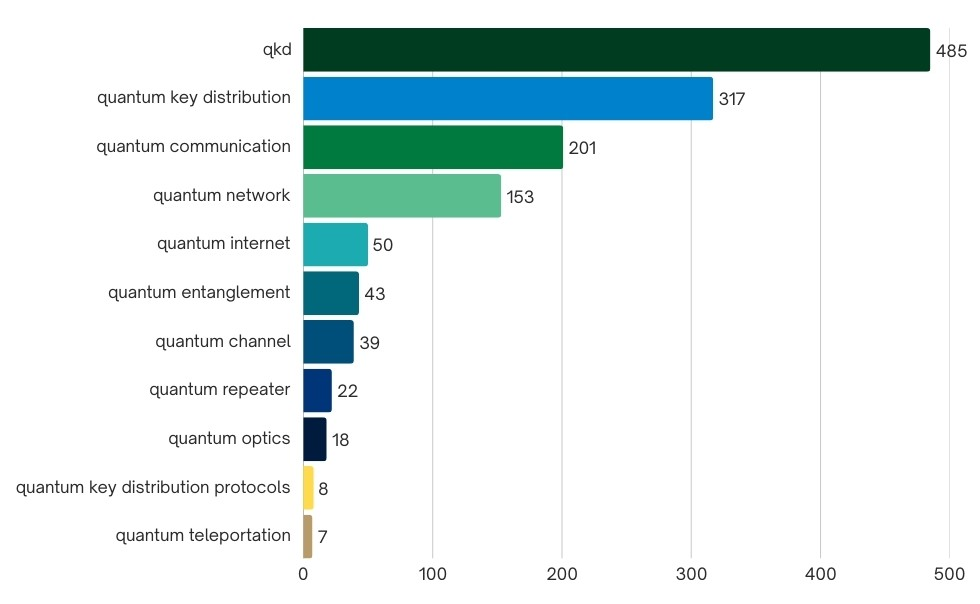
\includegraphics[width=0.90\textwidth]{pictures/Keywords_SLRCommunication.jpg}
\label{fig:keywords_com}
\end{figure}

A continuación, el tercer análisis busca reflejar el estado actual del campo e identificar que líneas presentan un mayor avance. Para ello, los artículos fueron organizados en distintas categorías temáticas según su título, descripción y palabras claves. Estas categorías temáticas representan las principales áreas de desarrollo dentro de las comunicaciones cuánticas.

\begin{itemize}
    \item \textbf{Quantum Key Distribution (QKD):} engloba protocolos, métodos y análisis de seguridad para la distribución de claves cuánticas.
    \item \textbf{Quantum Networks:} abarca arquitecturas y soluciones para interconectar nodos cuánticos, gestionar recursos y habilitar redes seguras, desde topologías metropolitanas hasta escenarios integrados con 5G/6G.
    \item \textbf{Quantum Communication Infrastructure:} incluye los desarrollos tecnológicos y experimentales necesarios para implementar estas redes, como fibras ópticas, enlaces físicos, hardware, fotónica, memorias, repetidores cuánticos.
    \item \textbf{Satellite \& Free-Space Quantum Communications:} reúne investigaciones en enlaces cuánticos espaciales y de espacio libre, mediante satélites y estaciones terrestres, considerando también efectos atmosféricos y entornos no guiados.
    \item \textbf{Quantum Internet \& Future Directions:} comprende visiones, propuestas en aplicaciones emergentes hacia un internet cuántico global, incluyendo integración con IA, blockchain, IoT y perspectivas futuras para la estandarización y despliegue.
\end{itemize}

\begin{figure}[H]
\centering
\caption[Artículos por campo de estudio - Comunicaciones Cuánticas]{
    \vspace{4pt}
    \fontsize{12}{11}\selectfont \\
    Artículos por campo de estudio - Comunicaciones Cuánticas \\
}
\footnotesize Fuente: Elaboración propia
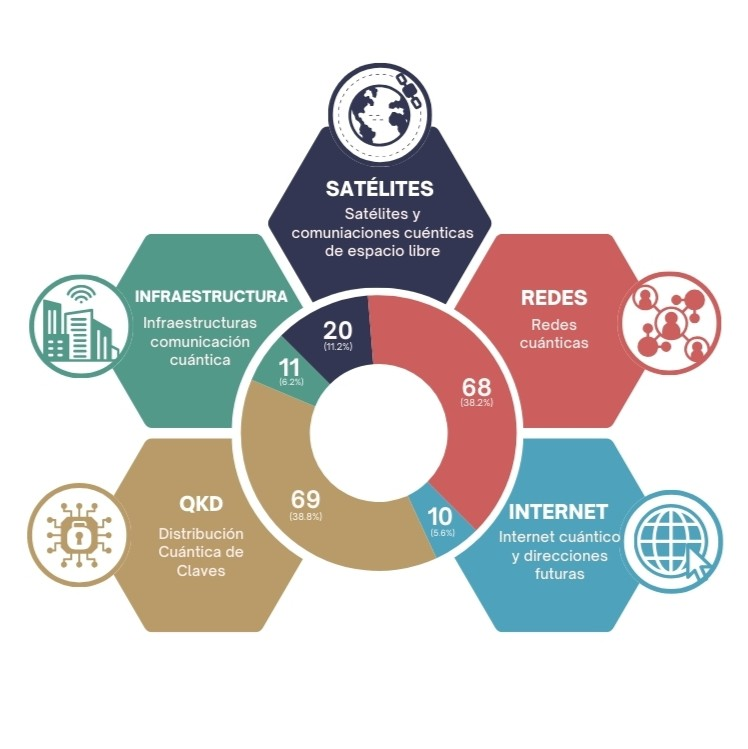
\includegraphics[width=0.90\textwidth]
{pictures/Campos_Estudio_SLRCommunication.jpg}
\label{fig:Campos_Estudio_SLRCommunication}
\end{figure}

Además, se realizó un último estudio centrado en identificar los artículos que han tenido un mayor impacto dentro de la comunidad científica. 

Por un lado, se presentan los diez artículos con mayor número de citaciones y por otro una gráfica comparativa por campos temáticos que permite visualizar que áreas dentro de las comunicaciones cuánticas han tenido una mayor atención y consolidación dentro de la literatura.

\begin{longtable}{@{} p{10.5cm} c @{}}
\caption[Artículos más citados - Comunicaciones Cuánticas]{
   \vspace{4pt}
   \fontsize{12}{11}\selectfont \\
   Artículos más citados - Comunicaciones Cuánticas\\[2pt]
}
\label{tab:articulos_mas_citados_comunicaciones_cuanticas}\\
\hline
\noalign{\vskip 2pt}
\hline
\textbf{Artículo} & \textbf{Citas} \\
\hline
\endfirsthead

\hline
\endhead

\hline
\endfoot

\hline
\noalign{\vskip 2pt}
\hline
\endlastfoot

The Evolution of Quantum Key Distribution Networks: On the Road to the Qinternet (2022)~\cite{Cao2022} & 431 \\
\hline
Breaking the Rate-Loss Bound of Quantum Key Distribution with Asynchronous Two-Photon Interference (2022)~\cite{Xie2022} & 239 \\
\hline
Concurrent Entanglement Routing for Quantum Networks: Model and Designs (2024)~\cite{Shi2024} & 211 \\
\hline
Quantum Internet protocol stack: A comprehensive survey (2022)~\cite{ILLIANO2022} & 202 \\
\hline
Full daylight quantum-key-distribution at 1550 nm enabled by integrated silicon photonics (2021)~\cite{Avesani2021} & 170 \\
\hline
Quantum-Enabled 6G Wireless Networks: Opportunities and Challenges (2022)~\cite{Wang2022} & 167 \\
\hline
Quantum Key Distribution Secured Optical Networks: A Survey (2021)~\cite{Sharma2021} & 130 \\
\hline
Implementation of a 46-node quantum metropolitan area network (2021)~\cite{ChenT2021} & 124 \\
\hline
Toward Practical Quantum Secure Direct Communication: A Quantum-Memory-Free Protocol and Code Design (2020)~\cite{Sun2020} & 104 \\
\hline
A Review of Quantum Key Distribution Protocols in the Perspective of Smart Grid Communication Security (2022)~\cite{Kong2022} & 102 \\
\end{longtable}


\begin{figure}[H]
\centering
\caption[Citaciones por campo de estudio - Comunicaciones Cuánticas]{
    \vspace{4pt}
    \fontsize{12}{11}\selectfont \\
    Citaciones por campo de estudio - Comunicaciones Cuánticas\\
}
\footnotesize Fuente: Elaboración propia
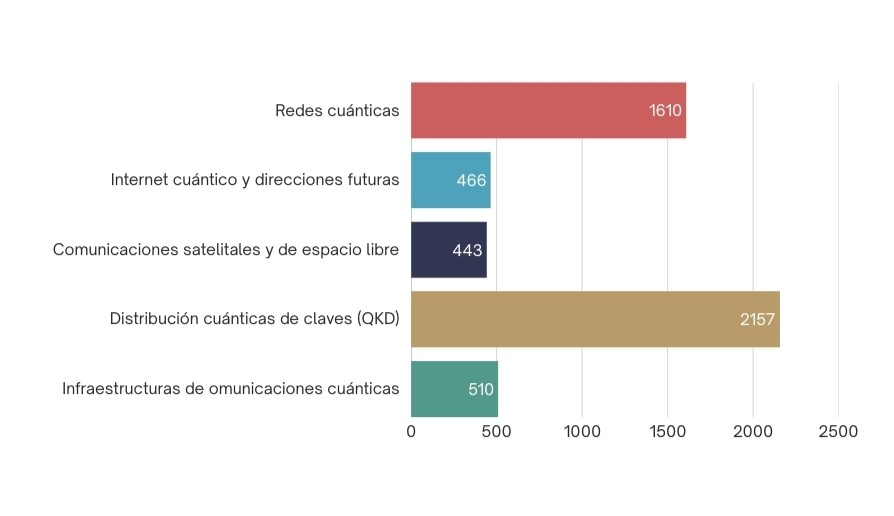
\includegraphics[width=0.95\textwidth]{pictures/Citas__SLRCommunication.jpg}
\label{fig:Citas_SLRCommunication}
\end{figure}

\section{Análisis Preguntas de Investigación}

Con el propósito de ofrecer una respuesta a los objetivos de investigación planteados en esta revisión sistemática, a continuación se presenta una tabla para cada pregunta con algunos de los artículos que aportan evidencia o contribución relevante.

\vspace{1em} \textbf {Q1: ¿Qué tecnologías, arquitecturas y protocolos constituyen el estado del arte actual de las comunicaciones cuánticas?}

Esta pregunta tiene como objetivo explorar y resumir el estado actual de las comunicaciones cuánticas. Se busca identificar las tecnologías más avanzadas, las arquitecturas implementadas y los protocolos que hacen posible su funcionamiento. Con esto, se espera construir una visión integral que ayude a entender en qué etapa se encuentra la investigación y cuáles son los referentes tecnológicos que marcan la dirección de este campo.

\begin{longtable}{@{} p{4.5cm} p{6.5cm} c c @{}}
\caption[Q1 - Comunicaciones Cuánticas]{
  \vspace{4pt}
  \fontsize{12}{11}\selectfont \\
   Q1 - Comunicaciones Cuánticas \\[2pt]
}
\label{tab:q1_slr_SLRcomunica}\\
\hline 
\noalign{\vskip 2pt} 
\hline
\textbf{Artículo} & \textbf{Descripción} & \textbf{Año} & \textbf{Citas} \\
\hline 
\endfirsthead
\hline
\endhead
\hline
\endfoot
\hline 
\noalign{\vskip 2pt} 
\hline
\endlastfoot

A review of quantum communication and information networks with advanced cryptographic applications using machine learning, deep learning techniques~\cite{RAMYA2025} & Revisa redes de comunicación cuántica, tecnologías clave (QKD, repetidores, memoria), el rol de la IA/ML, y la visión de la Internet Cuántica y sus aplicaciones. & 2025 & 5 \\
\hline
Integrating Quantum and Satellites: A New Era of Connectivity~\cite{Sodagari2023} & Explora el networking cuántico satelital, esquemas QKD (variable continua/discreta), selección de órbitas y la integración con redes definidas por software, incluyendo el papel de la computación cuántica. & 2023 & 5 \\
\hline
Quantum Key Distribution for 5G Networks: A Review, State of Art and Future Directions~\cite{Adnan2022} & Revisa el estado del arte de la criptografía cuántica para redes 5G, incluyendo protocolos, funcionalidad e implementaciones, e identifica brechas de investigación. & 2022 & 30 \\
\hline
The Evolution of Quantum Key Distribution Networks: On the Road to the Qinternet~\cite{Cao2022} & Repasa el desarrollo y la implementación de redes QKD, su arquitectura, elementos, interfaces y protocolos, además de soluciones de capa física/red y estandarización. & 2022 & 431 \\
\hline
Quantum Communication Systems: Vision, Protocols, Applications, and Challenges~\cite{Hasan2023} & Describe fundamentos, visión, protocolos, y el modelo de sistemas de comunicación cuántica, explorando aplicaciones y desafíos de la tecnología cuántica. & 2023 & 56 \\
\hline
Spooky action at a global distance: analysis of space-based entanglement distribution for the quantum internet~\cite{Khatri2021} & Propone una Internet Cuántica global mediante satélites para distribución de entrelazamiento, analizando configuraciones óptimas y tasas de distribución. & 2021 & 88 \\
\hline
The road to quantum internet: Progress in quantum network testbeds and major demonstrations~\cite{LIU2025} & Resume el progreso de redes cuánticas, destacando demostraciones y logros clave hacia la Internet Cuántica, y discute desafíos futuros & 2025 & 6 \\
\hline
A Vision, Survey, and Roadmap Toward Space Communications in the 6G and Beyond Era~\cite{Ntontin2024} & Ofrece una visión y hoja de ruta para las comunicaciones espaciales post-2030, cubriendo sistemas satelitales con IA y redes cuánticas espaciales. & 2025 & 17 \\
\hline
A Comprehensive Study on Quantum Key Distribution Protocols~\cite{Mummadi2024} & Proporciona un estudio exhaustivo de los protocolos QKD, modelos de seguridad, implementaciones prácticas, avances y desafíos en repetidores y arquitecturas de red. & 2024 & 4 \\
\hline
Advanced QKD Protocols and Practical Challenges~\cite{Rajpurohit2024} & Se centra en protocolos QKD avanzados (MDI, TF-QKD), sus desafíos de implementación, técnicas de aleatorización de fase y el diseño de sistemas QKD con FPGA. & 2024 & 1 \\
\end{longtable}

\vspace{1em} \textbf {Q2: ¿Cuáles son los principales desafíos tecnológicos y físicos que dificultan el despliegue a gran escala de redes de comunicación cuántica?}

Se pretende examinar las limitaciones que dificultan que las comunicaciones cuánticas se conviertan en una realidad práctica a gran escala. Factores como la pérdida de señal en distancias largas , la necesidad de repetidores cuánticos, la estabilidad de los estados cuánticos o las limitaciones de la infraestructura actual son algunos de los aspectos fundamentales. Comprender estas barreras ayudará a identificar que avances científicos y tecnológicos son esenciales para lograr un despliegue masivo.

\begin{longtable}{@{} p{4.5cm} p{6.5cm} c c @{}}
\caption[Q2 - Comunicaciones Cuánticas]{
  \vspace{4pt}
  \fontsize{12}{11}\selectfont \\
   Q2 - Comunicaciones Cuánticas \\[2pt]
}
\label{tab:q2_slr_SLRcomunica}\\
\hline 
\noalign{\vskip 2pt} 
\hline
\textbf{Artículo} & \textbf{Descripción} & \textbf{Año} & \textbf{Citas} \\
\hline 
\endfirsthead
\hline
\endhead
\hline
\endfoot
\hline 
\noalign{\vskip 2pt} 
\hline
\endlastfoot

Investigation of the Atmospheric Optical Disturbances Impact on the Free Space Optics Quantum Key Distribution~\cite{Pchelkina2024} & Presenta un simulador de canal atmosférico para FSO-QKD, analizando factores como aerosoles, temperatura y pérdidas de potencia láser, que afectan el rendimiento de la distribución de clave. & 2024 & 9 \\
\hline
Homodyne Detection Quadrature Phase Shift Keying Continuous-Variable Quantum key Distribution with High~\cite{Liu2021} & Aborda la baja tolerancia al ruido excesivo y la insuficiente distancia de transmisión en CV-QKD, proponiendo un protocolo para mejorar la tolerancia al ruido. & 2021 & 98 \\
\hline
Atmospheric Effects on Satellite-to-Ground Quantum Key Distribution using Coherent States~\cite{Villasenor2020} & Estudia la viabilidad de CV-QKD satelital a tierra usando estados coherentes, simulando la turbulencia atmosférica y determinando las tasas de clave QKD bajo estas condiciones. & 2020 & 34 \\
\hline
Effect of noise and topologies on multi-photon quantum protocols~\cite{Jha2024} & Investiga el impacto del ruido de canal y dispositivo, así como de las topologías de red, en los protocolos cuánticos multifotón, destacando sus ventajas sobre los protocolos de fotón único. & 2024 & 5 \\
\hline
Efficient Routing for Quantum Key Distribution Networks~\cite{Amer2020} & Modela el rendimiento del protocolo QKD E91 en redes con repetidores cuánticos y nodos confiables, proponiendo protocolos de enrutamiento para mejorar las tasas de comunicación segura. & 2020 & 63 \\
\hline
Time-Interleaved C-Band Co-Propagation of Quantum and Classical Channels~\cite{Wang2024} & Demuestra una técnica de entrelazado temporal para permitir la coexistencia de canales cuánticos y clásicos, mitigando el ruido de dispersión espontánea para el despliegue comercial. & 2024 & 10 \\
\hline
Proposal for space-borne quantum memories for global quantum networking~\cite{Gundogan2021} & Analiza el uso de satélites equipados con memorias cuánticas para la comunicación cuántica global, superando la pérdida exponencial de las fibras ópticas y aumentando las tasas de clave. & 2021 & 97 \\
\hline
Quantum Key Distribution in Multiple Fiber Networks and Its Application in Urban Communications: A Comprehensive Review~\cite{Granados2025} & Revisa la QKD en redes de fibra múltiples y su aplicación en comunicaciones urbanas, abordando desafíos como la pérdida de transmisión, perturbaciones ambientales y escalabilidad de la red. & 2025 & 0 \\
\hline
Hardware routed quantum key distribution networks~\cite{Singal2022} & Propone un esquema de redes de comunicación cuántica enrutadas por hardware para superar problemas de escalabilidad y ataques en las Redes Definidas por Software (SDN), mejorando la tasa de clave y utilización de recursos. & 2022 & 9 \\
\hline
FSO-QKD protocols under free-space losses and device imperfections: a comparative study~\cite{Sisodia2024} & Compara el rendimiento de protocolos QKD basados en fotones únicos y entrelazados bajo pérdidas de espacio libre e imperfecciones del dispositivo para comunicación terrestre. & 2024 & 5 \\
\end{longtable}

\vspace{7em} \textbf {Q3: ¿Qué impacto potencial tienen las comunicaciones cuánticas en el desarrollo de las infraestructuras de comunicación, y en qué medida podrían transformar los fundamentos tecnológicos que rigen las comunicaciones actuales?}

El propósito de esta cuestión es explorar el impacto disruptivo de las comunicaciones cuánticas, más allá de la seguridad. Se busca entender cómo estas tecnologías podrían transformar los cimientos arquitectónicos, operativos y de escalabilidad de las infraestructuras de comunicación, dando paso a nuevas maneras de interconexión global. 

\begin{longtable}{@{} p{4.5cm} p{6.5cm} c c @{}}
\caption[Q3 - Comunicaciones Cuánticas]{
  \vspace{4pt}
  \fontsize{12}{11}\selectfont \\
   Q3 - Comunicaciones Cuánticas \\[2pt]
}
\label{tab:q3_slr_SLRcomunica}\\
\hline 
\noalign{\vskip 2pt} 
\hline
\textbf{Artículo} & \textbf{Descripción} & \textbf{Año} & \textbf{Citas} \\
\hline 
\endfirsthead
\hline
\endhead
\hline
\endfoot
\hline 
\noalign{\vskip 2pt} 
\hline
\endlastfoot

Quantum-Driven Hybrid Network Architecture Leveraging 5G for High-Speed and Resilient Data Transmission~\cite{Kumar2025} & Propone una arquitectura de red híbrida cuántico-5G que usa QKD para seguridad y 5G para velocidad, mejorando rendimiento y seguridad en futuras redes de comunicación. & 2025 & 0 \\
\hline
Integrating Quantum-Secured Blockchain Identity Management in Open RAN for 6G Networks~\cite{Zeydan2024} & Propone la integración de QKD y blockchain para redes 6G, mejorando la seguridad y gestión de identidades y transformando las telecomunicaciones hacia un paradigma más seguro y descentralizado. & 2024 & 11 \\
\hline
MadQCI: a heterogeneous and scalable SDN-QKD network deployed in production facilities~\cite{Martin2024} & Presenta una red QKD escalable diseñada para flexibilidad e integración en ecosistemas de telecomunicaciones, abordando el despliegue práctico en infraestructuras existentes. & 2024 & 41 \\
\hline
Flexible entanglement-distribution network with an AlGaAs chip for secure communications~\cite{Appas2021} & Demuestra una red de distribución de entrelazamiento reconfigurable mostrando una ruta prometedora para el despliegue de arquitecturas de red cuántica rentables. & 2021 & 86 \\
\hline
QLSN: Quantum key distribution for large scale networks~\cite{MANGLA2024} & Propone un protocolo de gestión de claves inspirado en QKD para redes a gran escala, mejorando la seguridad y fiabilidad de la red al reemplazar métodos de intercambio de claves clásicos. & 2024 & 17 \\
\hline
Quantum Cryptography in 5G Networks: A Comprehensive Overview~\cite{Mehic2024} & Revisa la criptografía cuántica en redes 5G, abordando desafíos de seguridad, arquitecturas de red QKD y su integración en marcos de seguridad existentes para transformar las telecomunicaciones. & 2024 & 86 \\
\hline
QFMLNet: An AI-Driven Quantum Communication Architecture for 6G Space-Ground Networks~\cite{Ding2025} & Propone una arquitectura de comunicación cuántica impulsada por IA para redes 6G espacio-tierra, prometiendo velocidades sin precedentes, baja latencia y conectividad segura mejorada con QML y QFL. & 2025 & 0 \\
\hline
Towards metropolitan free-space quantum networks~\cite{Krzic2023}& Defiende las redes cuánticas de espacio libre como una alternativa práctica y eficiente para aplicaciones metropolitanas, complementando la infraestructura de fibra y facilitando la conectividad urbana. & 2023 & 30 \\
\hline
AirQKD: The Role of Free-Space Optics Quantum Key Distribution Enabling Pragmatic Secure and Scalable Communications~\cite{Davidson2024} & Destaca el papel de la FSO-QKD para la conectividad segura a escala metropolitana, como una solución complementaria a las redes 5G para mejorar la seguridad. & 2024 & 14 \\
\hline
Artificial Intelligence in Quantum Communications: A Comprehensive Survey~\cite{Mahmud2025} & Ofrece una visión general de cómo la IA puede mejorar la transmisión de datos, la corrección de errores y la escalabilidad en redes cuánticas, transformando los sistemas de comunicación para hacerlos más resilientes y adaptativos. & 2025 & 5 \\
\end{longtable}

\vspace{1em} \textbf {Q4: ¿Cuáles son los casos de uso industriales relevantes para las comunicaciones clásicas y cuánticas?}

La finalidad es identificar aplicaciones concretas que puedan impulsar la adopción de las comunicaciones cuánticas en sectores industriales estratégicos y mostrar aplicaciones reales saliendo de simples anotaciones teoricas o simulaciones de laboratorio. Ejemplos como la banca, la defensa, las infraestructuras críticas o el sector espacial representan escenarios donde la incorporación de estas tecnologías tendría un valor diferencial. Este análisis permitirá vincular el avance científico con la práctica industrial, subrayando el impacto real y las oportunidades de mercado.

\begin{longtable}{@{} p{4.5cm} p{6.5cm} c c @{}}
\caption[Q4 - Comunicaciones Cuánticas]{
  \vspace{4pt}
  \fontsize{12}{11}\selectfont \\
   Q4 - Comunicaciones Cuánticas \\[2pt]
}
\label{tab:q4_slr_SLRcomunica}\\
\hline 
\noalign{\vskip 2pt} 
\hline
\textbf{Artículo} & \textbf{Descripción} & \textbf{Año} & \textbf{Citas} \\
\hline 
\endfirsthead
\hline
\endhead
\hline
\endfoot
\hline 
\noalign{\vskip 2pt} 
\hline
\endlastfoot

QKD terminal for Canada’s Quantum Encryption and Science Satellite (QEYSSat)~\cite{Podmore2019} & Describe el desarrollo de un terminal QKD satelital para la misión QEYSSat de Canadá, buscando distribuir claves seguras para la transferencia de datos sensibles a largas distancias. & 2021 & 18 \\
\hline
On The Use of Quantum Communications for Securing IoT Devices in the 6G Era~\cite{AlMohammed2021} & Propone y simula un nuevo enfoque de QKD para proteger dispositivos IoT y cifrar datos enviados a servidores, demostrando su eficiencia y aplicabilidad en la seguridad de IoT. & 2021 & 53 \\
\hline
Madrid Quantum Communication Infrastructure: A testbed for assessing QKD technologies into real production networks~\cite{Lopez2021} & Reporta sobre la infraestructura de comunicación cuántica de Madrid, demostrando la integración de QKD en redes de telecomunicaciones de producción con casos de uso relevantes. & 2021 & 21 \\
\hline
Deploying an Inter-European Quantum Network~\cite{Ribezzo2023} & Describe la implementación de la primera red cuántica que conecta tres países diferentes utilizando fibra óptica existente haciendo uso de la tecnología QKD. & 2023 & 86 \\
\hline
QUARC: Quantum Research Cubesat-A Constellation for Quantum Communication~\cite{Mazzarella2020} & Propone una constelación de 15 CubeSats para formar una red troncal de comunicación cuántica segura para redes terrestres y metropolitanas. & 2020 & 88 \\
\hline
Towards the industrialisation of quantum key distribution in communication networks: A short survey~\cite{Liu2022} & Revisa las aplicaciones potenciales de la QKD para futuras tecnologías de comunicación, destacando los esfuerzos de estandarización y los desafíos para su implementación en diversas industrias. & 2022 & 89 \\
\hline
Metropolitan Quantum-Drone Networking and Computing: A Software-Defined Perspective~\cite{Chiti2022} & Explora el uso de enjambres de drones para crear redes cuánticas metropolitanas, habilitando aplicaciones de computación cuántica distribuida y servicios QKD en entornos donde la fibra es limitada. & 2022 & 22 \\
\hline
The European Satellite-Based QKD System EAGLE-1~\cite{Hiemstra2025} & Reporta sobre el estado y la contribución de Tesat-Spacecom a la misión satelital EAGLE-1, un paso importante hacia una futura red pan-europea de QKD segura. & 2025 & 1 \\
\hline
UAV-Assisted Quantum Key Distribution for Secure Communications With Resource Limited Devices~\cite{Kong2024} & Propone el uso de drones para distribuir claves cuánticas, permitiendo comunicaciones seguras en dispositivos con recursos limitados y en áreas sin canales cuánticos fijos. & 2024 & 11 \\
\hline
Implementation of a 46-node quantum metropolitan area network~\cite{ChenT2021} & Presenta la implementación de una red cuántica metropolitana que utiliza claves cuánticas para comunicaciones seguras en tiempo real, como voz, mensajería y transmisión de archivos. & 2021 & 124 \\
\end{longtable}

\section{Hallazgos y nuevas líneas futuras}

En esta investigación se ha podido observar como la evolución en las comunicaciones cuánticas es una realidad tecnológica que abre un abanico de posibilidades para el futuro de las infraestructuras de comunicación a nivel global~\cite{Hasan2023}.

Uno de los principales hallazgos es la consolidación y el uso real de la Distribución Cuántica de Claves (QKD es tal la madurez que ha adquirido que a día de hoy se está comenzando a implementar en redes metropolitanas y proyectos intercontinentales. Este hecho subraya la seguridad incondicional de la información que QKD ofrece gracias a los principios físicos de la cuántica, siendo una herramienta fundamental para contrarrestar las amenazas emergentes de la computación cuántica ante los sistemas criptográficos tradicionales.

Otro aspecto esencial es entender como las comunicaciones cuánticas no se están desarrollando de forma aislada. Por el contrario, buscan adaptarse al ecosistema tecnológico actual y futuros avances. Su propósito es aumentar las capacidades de las redes 5G, y próximamente 6G, la integración con otras tecnologías paralelas como blockchain o la inteligencia artificial todo ello con el objetivo de mejorar la seguridad, transmisión y eficiencia operativa de las redes. Escenarios cada vez más complejos y sofisticados que prometen una evolución significativa en la forma en que nos comunicamos. 
	
Las comunicaciones cuánticas, sin embargo, enfrentan aún grandes desafíos. La atenuación de la señal en fibras ópticas de larga distancia ha sido siempre una barrera que ha dificultando su integración en las infraestructuras de red actuales. Como consecuencia de esta limitación tecnológica se han impulsado diversos enfoques, entre los que destacan las redes cuánticas espaciales que buscan establecer enlaces satelitales a escala planetaria, esenciales para una futura internet cuántica global o la comunicación cuántica de espacio libre, que permite la transmisión de fotones directamente a través de la atmósfera, sin depender de la fibra óptica.
		
Mirando hacia el futuro, los esfuerzos deben concentrarse en lograr la estandarización de protocolos y componentes, requisito fundamental para garantizar la interoperabilidad entre redes y fabricantes. En paralelo, resulta crucial el desarrollo de repetidores cuánticos que permitan extender el alcance de las comunicaciones y sentar las bases de una conectividad cuántica segura extremo a extremo sin la necesidad de operar con nodos de confianza intermedios. Este avance junto con el uso eficiente de enlaces satelitales será clave para superar las barraras geográficas y asegurar la resiliencia y robustez ante desafíos físicos y ambientales. Además, se espera un perfeccionamiento y optimización energética de las fuentes de fotones así como la mejora de detectores y sistemas que faciliten la coexistencia fluida de canales cuánticos y clásicos en la misma infraestructura. Todos estos progresos, que podrían hacerse realidad en menos de diez años, serán determinantes para la adopción generalizada de las comunicaciones cuánticas.
